% CG-Tutor -- 2026 Spring Computer Graphics Project 3
% Compile with: cd report && pdflatex main && bibtex main && pdflatex main && pdflatex main

\documentclass[10pt,letterpaper]{article}

\usepackage[margin=1in]{geometry}
\usepackage[T1]{fontenc}
\usepackage{lmodern}
\usepackage{microtype}
\usepackage{amsmath,amssymb}
\usepackage{graphicx}
\usepackage{booktabs}
\usepackage{xcolor}
\usepackage[hidelinks]{hyperref}
\usepackage[round,authoryear]{natbib}
\usepackage{enumitem}
\usepackage{caption}
\usepackage{subcaption}
\usepackage{float}
\usepackage{authblk}

\hypersetup{
  colorlinks=true,
  linkcolor=blue!50!black,
  citecolor=blue!50!black,
  urlcolor=blue!70!black,
}

\newcommand{\github}{\url{https://github.com/AssassinCow/CG-PJ3.git}}

\title{\bfseries CG-Tutor: Agentic Generation and Verification of\\
3D Educational Animations for Computer Graphics}

\author[1]{Liu Zhuoxin, 24300240170}
\author[1]{Zhu Jinzhou, 24300240117}
\affil[1]{Fudan University, Computer Graphics 2026 Spring Project 3}

\date{}

\begin{document}
\maketitle

\begin{abstract}
We present \textbf{CG-Tutor}, an agentic framework that turns a compact
computer-graphics concept specification into a rendered Blender teaching
animation with structured diagnostics. The system combines language-model
agents for decomposition, scene profiling, storyboarding, Blender code
generation, and render critique with deterministic verification layers:
Auto Success Spec, Scene IR, visual contracts, static scene verification,
preview checks, concept metrics, critic--AST cross-reference, repair
planning, and conservative best-of-N selection. Unlike a one-shot prompt
pipeline, CG-Tutor treats ``success'' as an intermediate object that must
survive narrative planning, code generation, preview rendering, critic
feedback, and final selection. In the current repository snapshot we
retain five generated concept videos: affine transformation, forward
kinematics, mirror reflection, prism dispersion, and shape morphing. All
five produce final videos and replayable artifacts, but all are honestly
marked \texttt{best\_with\_violations}; this reflects the framework's
current design choice not to misreport visually plausible but semantically
incomplete results as passes. The main lesson is that reliable educational
generation needs evidence-preserving feedback loops, not merely longer
prompts or more scene-specific rules. \textbf{Code:}~\github.
\end{abstract}

\section{Introduction}

Computer graphics concepts are inherently spatial and temporal. Students
understand an affine transform, a kinematic chain, a reflected ray, or a
dispersion path by seeing how objects, coordinate frames, vectors, and
labels move together. Hand-authoring such animations in Blender or Manim is
effective but expensive, and the cost grows quickly across a course
curriculum.

Large language models can write Blender Python, but a direct
``concept-to-code'' prompt is brittle. During this project we repeatedly
observed that syntactically correct code and visually pleasant frames do
not imply pedagogical correctness: labels can be mirrored, rays can be
missing, helper objects can dominate the view, and a video can render while
failing the intended concept. The final version of CG-Tutor therefore
focuses less on one-shot generation and more on a closed feedback chain:
success criteria are generated, checked, criticized, cross-referenced
against code, and fed back into the coder as bounded repair targets.

\paragraph{Contributions.}
\begin{enumerate}[leftmargin=*,topsep=2pt,itemsep=2pt]
  \item A multi-agent Blender animation pipeline for computer-graphics
        teaching concepts, from YAML input to final MP4 and replayable
        \texttt{scene.py}.
  \item An automatic Success Spec layer that derives soft, machine-readable
        expectations from ordinary concept/storyboard tokens, without
        requiring users to hand-write per-scene metrics.
  \item A verification and feedback stack that combines static code checks,
        visual contracts, preview rendering, critic ensemble reports,
        deterministic metrics, and critic--AST cross-reference.
  \item A conservative selection policy that separates structural failures,
        hard success failures, soft success evidence, and aesthetic warnings,
        preventing high visual scores from masking semantic violations.
  \item A current empirical snapshot of five retained concept runs, including
        both successful rendering and explicit failure accounting.
\end{enumerate}

\section{Related Work}

\paragraph{Agentic 2D and presentation generation.}
GenPilot performs test-time prompt optimization for image generation by
detecting and repairing semantic errors~\citep{genpilot2025}. Paper2Poster
and PosterForest decompose scientific poster generation into parsing,
planning, layout, and feedback agents~\citep{paper2poster2025,posterforest2025}.
PresentAgent targets document-to-presentation video generation with slide,
narration, and composition agents~\citep{presentagent2025}. CG-Tutor shares
their decomposition mindset but targets executable 3D animation rather than
static or slide-based media.

\paragraph{Agentic 3D generation.}
LL3M reframes text-to-3D modeling as writing modular Blender Python
code~\citep{ll3m2025}. CAD-Assistant uses a VLLM planner with CAD tools for
parametric modeling tasks~\citep{cadassistant2025}. SAGE uses agents to
generate physically plausible indoor scenes for embodied-AI
simulation~\citep{sage2026}. CG-Tutor is closest to LL3M in its use of
Blender code, but differs in objective: the output is not a standalone
asset or room, but a time-synchronized teaching explanation whose success
depends on visible relationships between objects, labels, vectors, and
camera motion.

\paragraph{Agentic video systems.}
AniMaker builds long-form animated stories through director, camera,
review, and post-production agents~\citep{animaker2025}. CG-Tutor is smaller
in media scope but stricter in semantic structure: a ray, surface normal,
joint label, or transformation cue must be traceable through generated code
and rendered evidence.

\section{Method}
\label{sec:method}

\subsection{Overview}

\begin{figure}[H]
  \centering
  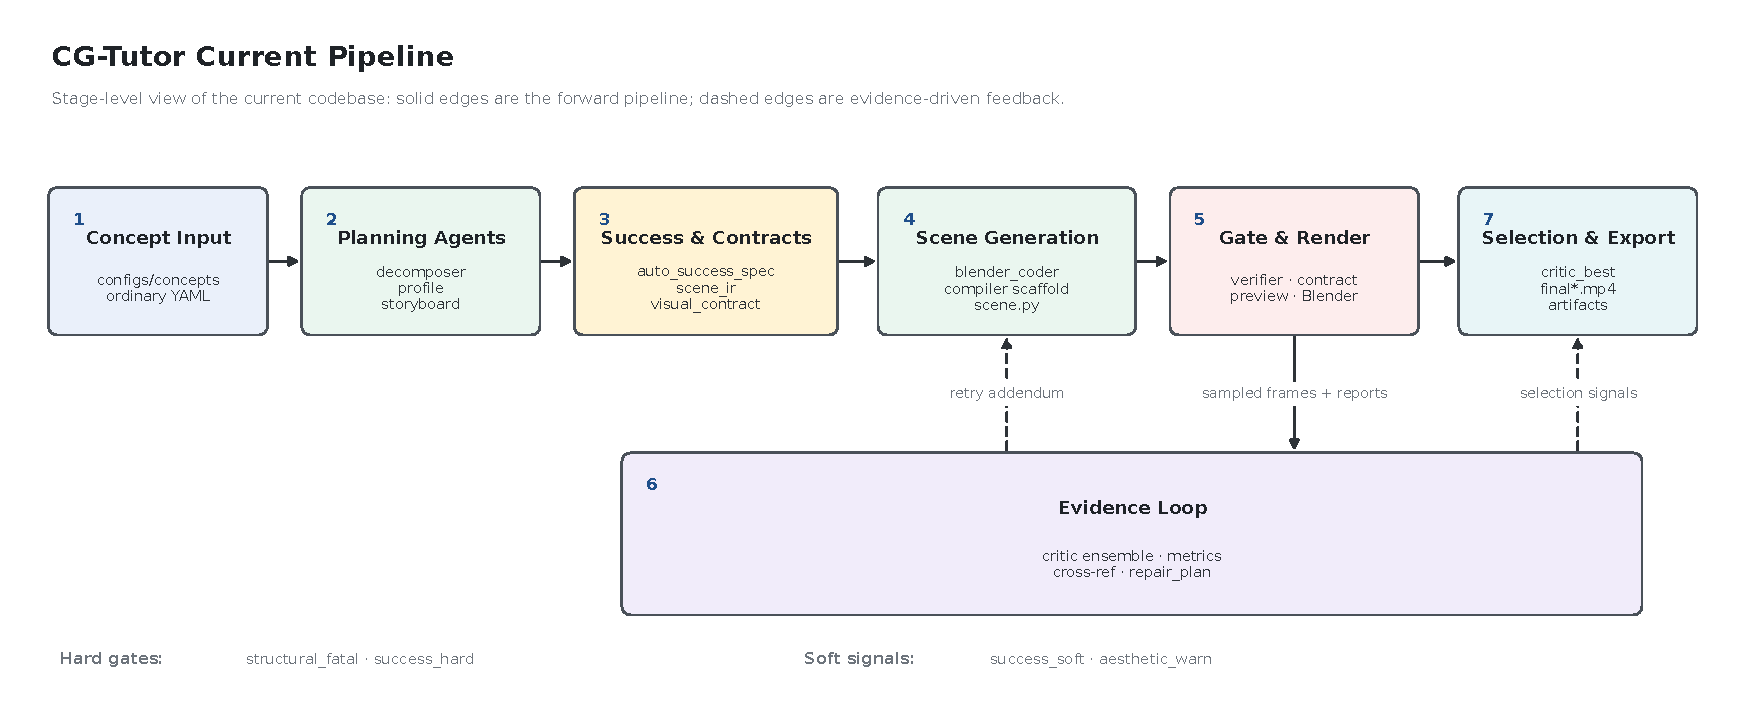
\includegraphics[width=0.93\linewidth]{figures/pipeline.pdf}
  \caption{Current CG-Tutor pipeline. LLM agents propose narrative,
  profile, storyboard, and Blender code. Deterministic layers derive Auto
  Success Spec rules, Scene IR, visual contracts, compiled fallbacks,
  verifier reports, critic evidence, and repair targets before selecting
  the final video.}
  \label{fig:pipeline}
\end{figure}

The pipeline is organized around typed intermediate artifacts rather than
one large prompt. A concept YAML is decomposed into a narrative and scene
profile. From these and the storyboard, the system generates an Auto Success
Spec, Scene IR, visual contracts, and a deterministic compiled scaffold. The
Blender coder then emits \texttt{scene.py}. Before expensive rendering,
static verifier, contract validator, and preview checks reject or downgrade
unsafe candidates. After rendering, a critic ensemble and deterministic
metrics produce structured evidence for repair and best selection.

\subsection{Agent Roles and Data Flow}

\paragraph{Concept decomposition and scene profile.}
The decomposer converts the concept YAML into 2--5 narrative nodes with
durations, formulas, and concrete visual intent. The profile generator then
classifies the scene style and extracts persistent anchors, spatial
relationships, forbidden abstractions, and profile-specific constraints.
This matters for application-like concepts: without explicit anchors, a
``mirror reflection'' or ``prism dispersion'' prompt can collapse into
floating labels and abstract primitives.

\paragraph{Auto Success Spec.}
The Auto Success Spec layer converts available tokens from the concept,
profile, and storyboard into soft expectations such as
\texttt{object\_visible}, \texttt{text\_readable},
\texttt{stay\_in\_screen\_safe}, \texttt{helper\_hidden},
\texttt{animation\_coverage}, and \texttt{progressive\_visual\_ordering}.
Generated rules do not hard-fail the first iteration. They are used as
evidence for retry and selection, and can only become hard failures within
the current run when repeated critic evidence is not contradicted by static
code evidence.

\paragraph{Storyboard, Scene IR, and visual contracts.}
The storyboard agent creates shots, camera plans, objects, labels, formulas,
and timing. Deterministic sanitization then produces Scene IR and per-shot
visual contracts. Contracts encode required anchors, labels, vector cues,
and forbidden failures in a vocabulary that both verifier and critic can
reuse. This is especially important for vector/ray concepts, where the
presence of a generic line is not enough; object names and local visibility
must still preserve the intended teaching relationship.

\paragraph{Blender coder and compiled fallback.}
The LLM coder generates a self-contained Blender Python script. In parallel,
the deterministic compiler creates a scaffold from Scene IR. The scaffold is
not treated as a semantic success; it is a render-safe diagnostic fallback
when LLM code is non-renderable. Fallback outputs are explicitly marked as
degraded unless they also pass verifier, contract, critic, and metric checks.

\subsection{Verification and Feedback}

\begin{figure}[H]
  \centering
  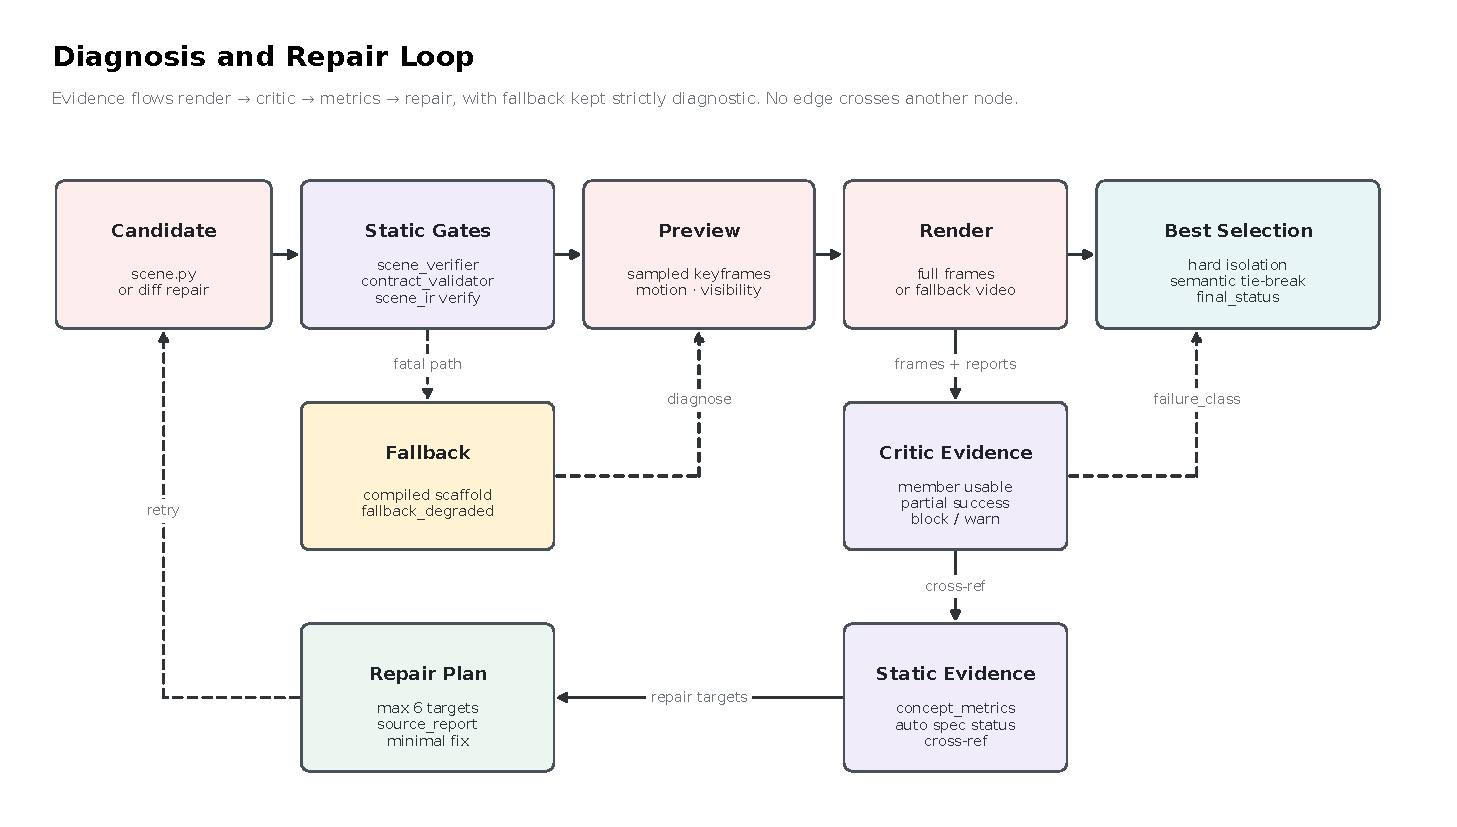
\includegraphics[width=0.88\linewidth]{figures/architecture_feedback_loop.pdf}
  \caption{Diagnostic loop. Static checks, preview evidence, critic reports,
  concept metrics, and critic--AST cross-reference are compressed into a
  bounded repair plan. The coder receives a small number of high-confidence
  targets instead of a raw issue dump.}
  \label{fig:feedback}
\end{figure}

\paragraph{Static and preview checks.}
The scene verifier checks render safety, syntax-level patterns, render calls,
engine setup, animation keyframes, text orientation evidence, and other
low-level hazards. The contract validator checks whether declared anchors,
labels, and vector geometry are present. Preview rendering samples a small
set of frames before full render to catch blank frames, missing motion, and
obvious crashes.

\paragraph{Critic ensemble and partial success.}
The render critic uses a Claude/GPT ensemble under strict or union
aggregation. A member report with useful issues is retained even if that
backend also has a parsing or execution diagnostic; only reports with errors
and no usable issues are discarded. This avoids a common failure mode where
the critic saw many real problems but retry received zero targets.

\paragraph{Repair plan and failure classes.}
Issues keep the legacy \texttt{block}/\texttt{warn} labels, but the final
selection logic also uses four failure classes:
\texttt{structural\_fatal}, \texttt{success\_hard},
\texttt{success\_soft}, and \texttt{aesthetic\_warn}. Repair planning
prioritizes fatal verifier and render-contract failures, then contract
structure, critic concept mismatch, cross-reference findings, and Auto
Success Spec evidence. Each retry is capped to a small number of
high-confidence targets to reduce Goodhart-style overfitting, such as adding
more labels instead of fixing an existing unreadable one.

\begin{figure}[H]
  \centering
  
\includegraphics[width=0.82\linewidth]{figures/architecture_module_layers.pdf}
  \caption{Module layering in the current codebase. The top-level pipeline
  coordinates agent calls, deterministic checks, render execution, and
  artifact export, while specialized modules own success specs, contracts,
  metrics, cross-reference, and repair planning.}
  \label{fig:layers}
\end{figure}

\subsection{Output Artifacts}

Each run stores the final videos plus replay artifacts: narrative,
storyboard, scene profile, generated/effective success specs, visual
contracts, scene code, compiled fallback, verifier reports, critic member
reports, repair plans, and \texttt{critic\_best.json}. This is intentional:
the current goal is not only to render a video, but to make failures
inspectable and reproducible.

\section{Experiments}
\label{sec:experiments}

\subsection{Evaluation Setup}

The retained repository snapshot contains one output root, \texttt{outputs/},
with five concepts. These runs use the current architecture, critic ensemble
feedback, verifier/contract checks, Auto Success Spec artifacts, and
conservative best selection. We report the best selected iteration, critic
score, issue counts, success-spec issue counts, and final status.

For each retained concept, the submitted artifacts include one primary
\texttt{final.mp4} and four selector-specific alternatives:
\texttt{final\_balanced.mp4}, \texttt{final\_compliance.mp4},
\texttt{final\_aesthetic.mp4}, and \texttt{final\_semantic.mp4}. The report
uses \texttt{final.mp4} as the main result and treats the alternatives as
diagnostic views of the same run rather than independent experiments.

\begin{table}[H]
\centering
\footnotesize
\setlength{\tabcolsep}{3.2pt}
\begin{tabular}{lcccccc}
\toprule
Concept & Best iter & Score & Frame b/w & Concept b/w & Success h/s & Final status \\
\midrule
\texttt{affine\_transformation} & 0 & 0.8125 & 0 / 4 & 7 / 12 & 0 / 0 & \texttt{best\_with\_violations} \\
\texttt{forward\_kinematics\_chain} & 1 & 0.7150 & 7 / 1 & 7 / 20 & 0 / 1 & \texttt{best\_with\_violations} \\
\texttt{mirror\_reflection} & 2 & 0.7750 & 0 / 2 & 16 / 15 & 0 / 1 & \texttt{best\_with\_violations} \\
\texttt{prism\_dispersion\_teaching} & 1 & 0.8388 & 0 / 8 & 1 / 18 & 0 / 0 & \texttt{best\_with\_violations} \\
\texttt{shape\_morphing} & 0 & 0.7625 & 1 / 6 & 3 / 14 & 0 / 1 & \texttt{best\_with\_violations} \\
\bottomrule
\end{tabular}
\caption{Current retained experiment snapshot. All five concepts render a
final MP4 and preserve diagnostic artifacts, but none is marked as strict
\texttt{pass}. This is a deliberate conservative policy: semantic or visual
evidence gaps remain visible instead of being hidden behind a scalar score.}
\label{tab:current-results}
\end{table}

\subsection{Case Observations}

\paragraph{Affine transformation.}
This concept is the most stable of the retained set. Its geometry is compact,
and the main challenge is legibility of axes, labels, and transformation
relationships rather than environment grounding. It shows that the current
pipeline can produce a coherent final video while still surfacing residual
concept issues.

\paragraph{Forward kinematics chain.}
Forward kinematics stresses hierarchical naming and joint semantics. The
system can render the articulated chain, but issue counts remain high because
end-effector, joint, and transform labels are easy to omit or misname.
This validates the need for cross-reference between critic findings and
scene-object creation, rather than relying on critic prose alone.

\paragraph{Mirror reflection.}
Mirror reflection is the most important stress test for the feedback loop.
It combines ray vectors, surface normals, angle relationships, labels, and
render-contract fragility. The current run reaches a renderable final video,
but its concept issue count remains high. This means the architecture can
diagnose the failure, but vector/ray spatial correctness is still not
reliably generated by the coder.

\paragraph{Prism dispersion teaching.}
Prism dispersion is the strongest visual sample in the retained set. The
optical-table metaphor, RGB rays, internal ray, and surface-normal cues are
well matched to the current scaffold and contract machinery. Its remaining
warnings show the difference between ``colored rays are present'' and
``dispersion geometry is fully pedagogically correct''.

\paragraph{Shape morphing.}
Shape morphing stresses temporal continuity. It is less dependent on complex
ray semantics, but it exposes another weakness: sparse keyframe checks do not
guarantee smooth interpolation over the full video. This points toward
render-evidence extraction as the next high-value direction.

\subsection{What the Experiments Show}

The five runs support three conclusions. First, the current architecture is
operational: it generates videos, stores replayable code, and preserves rich
diagnostics. Second, automatic feedback is useful but not magical: critic
evidence and static checks improve observability, yet the LLM coder still
struggles with precise vector/label relationships. Third, conservative final
status is necessary. Without \texttt{best\_with\_violations}, a visually
acceptable video could be mistaken for a correct teaching artifact.

\section{Discussion}
\label{sec:discussion}

\paragraph{Why not just write better concept prompts?}
Early experiments suggested that incomplete concept text was only part of
the problem. Natural language intent must be compiled into verifiable
constraints. For example, a scene can contain a text object but still show
mirrored or unreadable text; a camera can animate focus distance without
making focus pull visible; a prism scene can contain colored lines without
showing correct entry, internal, and exit relationships.

\paragraph{Why not hard-code metrics for every concept?}
Hand-written metrics help specific scenes, but they do not scale to ordinary
users. The final architecture therefore keeps generated Success Spec rules
soft by default, upgrades them only with repeated evidence and static
support, and avoids writing scene-specific hard gates into the concept YAML.
This reduces the risk of negative optimization where the model satisfies
rules by adding clutter rather than improving the teaching scene.

\paragraph{Remaining limitations.}
The largest limitation is still the generation side: if the first coded
scene lacks a clear semantic skeleton, repair often cannot fully rescue it.
The system also relies heavily on VLM critic judgment, which is useful but
not precise enough for all geometry. Future work should add render evidence
extractors for text readability, object visibility, safe-frame checks,
motion continuity, ray/normal geometry, and focus/blur changes.

\section{Conclusion}

CG-Tutor demonstrates a practical agentic workflow for generating
computer-graphics teaching animations in Blender. The strongest result is
not that every generated video passes; the stronger claim is that the system
can produce videos, preserve diagnostic artifacts, avoid overstating
success, and route failures back into bounded repair prompts. The project
also clarifies a broader lesson for agentic graphics systems: visual quality
and semantic success must be separated. Future progress should focus on
evidence extraction and stronger spatial relationship checks, not on
unbounded prompt growth or per-scene rule accumulation.

\bibliographystyle{plainnat}
\bibliography{references}

\appendix

\section{Reproducibility Notes}

The current repository snapshot keeps the retained videos and JSON/Python
diagnostic artifacts under \texttt{outputs/}. Historical frame snapshots
from earlier development are intentionally not part of the final report.
The architecture figures in this paper are generated by
\texttt{scripts/generate\_architecture\_figures.py}.

\section{Author Contributions}

\begin{itemize}[leftmargin=*,topsep=2pt,itemsep=2pt]
  \item Liu Zhuoxin: overall pipeline design, concept/storyboard/profile
        prompting, critic ensemble integration, Auto Success Spec design,
        experiment iteration, result analysis, and report organization.
  \item Zhu Jinzhou: Blender scene generation, Scene IR and compiled fallback,
        scene verifier and contract validation, render/runtime compatibility,
        concept metrics, critic--AST cross-reference, and evaluation
        packaging.
\end{itemize}

\end{document}
